% REMEMBER: You must not plagiarise anything in your report. Be extremely careful.

\documentclass{l4proj}

    
%
% put any additional packages here
%

\begin{document}

%==============================================================================
%% METADATA
\title{A Distributed Game Using Adverts and Trackers In Web Browsers}
\author{Eftychios Karagiorgis}
\date{March 14, 2021}

\maketitle

%==============================================================================
%% ABSTRACT
\begin{abstract}
    Every abstract follows a similar pattern. Motivate; set aims; describe work; explain results.
    \vskip 0.5em
    ``XYZ is bad. This project investigated ABC to determine if it was better. 
    ABC used XXX and YYY to implement ZZZ. This is particularly interesting as XXX and YYY have
    never been used together. It was found that  
    ABC was 20\% better than XYZ, though it caused rabies in half of subjects.''
\end{abstract}

%==============================================================================

% EDUCATION REUSE CONSENT FORM
% If you consent to your project being shown to future students for educational purposes
% then insert your name and the date below to  sign the education use form that appears in the front of the document. 
% You must explicitly give consent if you wish to do so.
% If you sign, your project may be included in the Hall of Fame if it scores particularly highly.
%
% Please note that you are under no obligation to sign 
% this declaration, but doing so would help future students.
%
%\def\consentname {My Name} % your full name
%\def\consentdate {20 March 2018} % the date you agree
%
\educationalconsent


%==============================================================================
\tableofcontents

%==============================================================================
%% Notes on formatting
%==============================================================================
% The first page, abstract and table of contents are numbered using Roman numerals and are not
% included in the page count. 
%
% From now on pages are numbered
% using Arabic numerals. Therefore, immediately after the first call to \chapter we need the call
% \pagenumbering{arabic} and this should be called once only in the document. 
%
% Do not alter the bibliography style.
%
% The first Chapter should then be on page 1. You are allowed 40 pages for a 40 credit project and 30 pages for a 
% 20 credit report. This includes everything numbered in Arabic numerals (excluding front matter) up
% to but excluding the appendices and bibliography.
%
% You must not alter text size (it is currently 10pt) or alter margins or spacing.
%
%
%==================================================================================================================================
%
% IMPORTANT
% The chapter headings here are **suggestions**. You don't have to follow this model if
% it doesn't fit your project. Every project should have an introduction and conclusion,
% however. 
%
%==================================================================================================================================
\chapter{Introduction}

% reset page numbering. Don't remove this!
\pagenumbering{arabic} 

Ad Tracking and targeted advertising are part of the web browsing eco-system. While it is not essential to the personal browsing experience of a user, it is the main source of income for businesses that provide free services (such as Facebook). With this model, users can in most cases browse the web for free, but this comes at the cost of the user's privacy, and usually without their knowledge. 

Online targeted advertising is done in a massive scale, and many entities are involved in this processes, having access to a large number of internet users. As a result, mass amounts of user data is is being transported between these entities. Adding to this the fact that there is a general lack of transparency on what exact data is gathered from the user and how it is processed, serious privacy concerns are constantly being expressed (cite something that expresses privacy issues in targeted advertising).
% TODO: Provide a bit more introduction to the project as well. Phrase the above paragrah a bit differently!

\section{Motivation}
The process of serving personalised adverts to the user starts from trackers that gather data about the user and share that data with advertisers. Advertisers then use that data to create an interest profile for users that is used to target personalised content in order to increase the likelihood that the user will be interested in their adverts with the hopes that the user will engage with that advert.

One of the privacy concerns with this process is that the user does not have much control over what data are used to create the interest profile or how the data are gathered, this leads into a very broad range of opinions and knowledge of targeted advertising systems.

In this paper, we attempt to use targeted advertising in a way that is fun and educational with the purpose of directly observing and improving the knowledge that users have of these systems. We also attempt to increase awareness of the various privacy and discrimination issues involved in these systems.
% TODO: Refine motivation section, mention briefly privacy issues in targeted advertsing, maybe also mention any scandals that happened, and then tie it up with what we are trying to do in this paper.

\section{Aims}
In order to investigate and improve user knowledge of targeted advertising systems, we create a mutli-player game using adverts and third-party trackers in web browsers as game entities. The nature of game is meant to be educational and experimental; We are not interested in building the most fun game, but rather explore the possibilities of using tracker and advertising as game mechanics. During the game-play, players can put their knowledge to the test, with the goal of tricking the profiling done by advertisers or getting tracked by a certain amount of ad trackers. 

In the first case, players are given an advert category that belongs to a content category (e.g Arts and Entertainment). Starting with a fresh browser account, they browse the web until they see an advert that belongs to the category given. This will allow the users to explore how the profiling is done by trying out different strategies to be targeted with an advert in that category. The first player to receive an advert in the given category is the winner. 

In the second case, the players browse the web with the goal to get tracked by a certain number of distinct third-party ad trackers. Third-party trackers can be found in almost all types of websites, but some websites have a lot more trackers than others, which means the players can devise strategies that maximise the number of trackers identified, which effectively means that they have gained some insight as to which websites contain the most trackers. The first player to get tracked by the required number of distinct third-party ad trackers wins.

The nature of the game being multi-player allow players to discuss and collaborate with each other, which increases the engagement with the game and makes things more interesting. It also introduces a competitive factor to the game that can act as a motivator for users to improve their strategies.  Additionally, after the game, players can see what websites the other players have visited, which will be a good starting point for new players to come up with their own strategies.

In addition to the game-play, we include information sections in the game which are meant to help with improving the user's knowledge of tracking and targeted advertising systems by providing the necessary context that the user needs to understand what is happening while they are playing the game.     

In both game modes, we gather relevant gameplay metrics in order to analyse and evaluate the player's strategies. Additionally, using surveys, we evaluate the player's knowledge of targeted advertising systems before and after playing the game as well as the usability of the system in general. In particular, for the users that played the game, the key questions we would like to explore are:
\begin{itemize}
    \item
    What did the user know about targeted advertising and what did they learn after playing the game?
    \item
    Did the user play the game blindly or did they have some sort of strategy in mind?
    \item
    If the user played multiple games, did their strategy improve over time?
\end{itemize}
% TODO: The Aims section is better to be left for after the evaluation. 

\section{Content Structure}
We begin in Chapter 2 by providing an overview of related technologies and the state of affairs in online targeted advertising. In Chapter 3, we formalise the requirements and discuss the different aspects of the required solution. Chapter 4 shows the design decisions made along with explanations, it also gives an overview of the process throughout the production of the product and includes a high level overview of the system architecture. Chapter 5 dives into the implementation of the product, where the abstract details given in Chapter 4 are explained in more detail. We split the independent components of the system and explain their functionality and various challenges encountered throughout the development, we then give a complete picture of the system by putting everything together. In Chapter 6, we describe our experiments with players and use the data gathered to make conclusions about the players understanding of targeted advertising systems. We also include a discussion on game engagement and the fun factor. Finally, in Chapter 7 we discuss the limitations of our product and set the groundwork for future work. We end with a conclusion on the findings of this paper and a discussion as to why users need to have a better understanding of online targeted advertising systems.
 % TODO: Ensure this section is correct when paper is finished


%==================================================================================================================================
\chapter{Background}
In this chapter we provide a discussion on the entities involved in targeted advertising and how it works, as well as how trackers collect the user's data. While we are mostly interested in third-party trackers for the purpose of our game, we also explain how first-party tracking is usually done. Furthermore, we explain briefly the privacy risks associated with targeted advertising and how they affects casual users. Finally, we explore technologies that are commonly used by users to deal with targeted advertising and we conclude with a section on related technologies to what we are trying to build.

\section{Early days of advertising}
Here talk about how advertising was done before we had access to so much data and machine learning techniques.

\section{Targeted advertising systems}
\label{targeted}
\subsection{Entities involved in targeted advertising systems and their roles}
Targeted advertising systems are complex and there are a lot of entities involved that interact with each other in order to serve personalised adverts to users. \cite{Estrada-Jimenez2017}, discuss in detail how these entities interact with each other and what implications this might have in terms of privacy issues. Abstracting those details, let us first begin by giving a brief and simplified overview of how these systems work. 

Ultimately, the goal of these systems is to deliver the right ads to the right users (cite). The entity responsible for promoting a service or product by serving ads to users are \textbf{advertisers}, but first they need a 'space' to display their advert so that they can maximise their reach of users. Typically, these spaces are provided by \textbf{publishers} and usually in the form of image banners in web pages with a redirection link to the website of the product or service being advertised. Publishers put these spaces on sale and they can either negotiate with advertisers to sell these spaces or have a real time auction to decide which advertiser is willing to give the best offer for a particular space at a particular point in time. It is through publishers that the users are exposed to the adverts. In practise, advertisers do not interact directly with the publishers but rather through ad platforms which provide interfaces that help advertisers and publishers improve their business plan and maximise their profit.

\textbf{Ad platforms} have evolved to make targeted advertising more efficient, transparent and flexible. This lead to more entities becoming involved to handle different parts of the systems. 

\textbf{Ad networks} are responsible for helping advertisers select the most optimal spaces for their adverts (an example of an ad network is GoogleAdSense).

\textbf{Ad exchanges} gather advert spaces from publishers and then using automated auctions, sell these spaces to the advertisers willing to pay the most. They also interact with the advertisers by sharing any data they have on the user that is currently being considered for a targeted advert, which is how the advertiser decides if they want to pay for a particular ad space or not. These auctions happen when the user is served content on a publisher's website and are extremely fast.

\textbf{Demand-side platforms (DSPs)} advise advertisers on what audience they should display their ads to and on what and platform. 

\textbf{Supply-side platforms (SSPs)} advise publishers on how to best use their spaces with the purpose of increasing profit and demand. 

Finally, \textbf{data aggregators} or trackers are the entities responsible for collecting information about the users by tracking their online activity, which they share with ad exchanges. Ad exchanges then provide this information to the demand and supply-side platforms.

\subsection{Collecting data}
\textbf{First-party tracking} is done by publishers, usually for the purpose of collecting and analysing the user's information to offer a better experience with using their website. First-party tracking involves tracking the user using first-party cookies, which the user has to give consent before they could be used for advertising purposes. Cookies usually capture implicit data about the user's interactions with the website. Furthermore, data provided by the user, either directly through forms or captured from their network requests are also gathered.

\textbf{Third-party tracking} involves tracking the user by embedding content in first party websites (i.e in publisher sites) that allows trackers to monitor the user's browsing activity and capture meaningful data that will later on be used to target the user with personalised content. This content is usually embedded in the website without the user's consent, and in most cases, without the user's knowledge.
First-party tracking is less of a privacy concern than third-party tracking as it is limited to the users that use the publisher's website. Additionally, there is usually more transparency as to what data is gathered and how it is used. The privacy risks in first-party tracking are directly corellated with the publisher's intentions; publishers can choose to sell private data to ad exchanges. Third-party tracking on the other hand is a much bigger privacy concern due to the lack of transparency and lack of user involvement. Finally, third-party trackers share the user's data with other entities in the targeted advertising eco-system, considering there is a vast amount of data moving between these entities, any potential data leaks can cause serious privacy issues. 
% TODO: maybe mention that trackers can combine data they have about the user, and why this is problematic 

\subsection{Process of serving personalised adverts to the user}
From the user's perspective, the ads that they see are part of the website they are visiting. The ads are indeed embedded in the content of the website, but the ads come from third parties, and are served when the user's browser sends an HTTP request to a publisher's website. Since publishers are directly associated with ad exchanges, along with the original content that the user would have been served, additional content is served in the form of scripts or ad tags which is executed automatically by the browser. The scripts automatically notify the ad exchange, which in turn notify advertisers that a space for adverts is available to be filled. Additionally, using cookie matching, ad exchanges can provide data about the user to the advertisers, and the ad space is then sold to the advertisers willing to pay the most, usually in real-time auctions in a process called real-time bidding (\cite{Estrada-Jimenez2017}).

This is a simplified view of how users get targeted with personalised adverts. In reality, many more of the entities mentioned in section \nameref{targeted} are involved in this process, with the ultimate goal of optimising the advertiser's and publisher's profit as well as maximising the perceived interest of the user for the advert to be served.

\subsection{Cookie Matching}
What is cookie matching and how does it work? 

\subsection{Real-time bidding (RTB)}
Explain the process of real-time bidding

\subsection{Privacy issues}
Private data being mined, lack of control and transparency that users have on how these systems work and what data is used, discrimination between user groups

\subsection{Discrimination Issues}
Briefly provide examples of discrimination in targeted advertising systems and why this is an issue. 

\section{Web categorisation}
 Why is this being mentioned? What can someone figure out by using this service?
Web categorisation is the process of classifying a website's content into a set of categories. This usually works by training a classification model that takes as input the html content of the website. There are a lot of services that provide web categorisation APIs, which allow you to make HTTP requests to categorise a website by including the website's url in the request. There are some limitations to these services however, as some websites might be difficult to classify because of complex content.

\section{Seams?}
Can adverts be seen as seams in a browsing experience? Not in the traditional sense, as seams are more seen as aspects of a system that are often hidden from users to provide a more smooth experience. In this area of seams, there is usually some form of technical understanding that a user must have to interact more efficiently with the system

\section{Related products}
\subsection{Tally Saves The Internet Game}
Explain what this is, when it came out and how similar it is to what we are trying to do. Conclude on why our project is different and why it is also usefull

\subsection{Adblockers}
Users receive adverts as HTTP content through HTTP requests. The requests are made when a user accesses a publisher's site, and are out of the users control. This lead to the development of browser add-ons that listen to these requests and block them, effectively blocking adverts from being served to the user. 

Ad blockers usually work by monitoring the user's HTTP traffic, and looking at the url of the domain that each request is made at. This url is then compared to a list that contains known advertiser domains and is either flagged as an advert or not, depending if the url is found in the list (an example of such a list is the EasyList). Alternatively, a domain can be flagged as an advert by identifying key words in the domain url. If the url is flagged as an advert, the ad blocker will block that request, which means the ad content will not be served to the user. Some ad blockers such as the AdBlockPlus chrome extension allow blocking additional traffic, where in addition to blocking requests made to known advert domains, they also block requests made to known tracker domains, which stops trackers from collecting the user's browsing activity. We will be using a similar technique in our game to identify trackers; but instead of blocking them, we simply count them.

Ad blockers are commonly used to block adverts that disrupt the user's browsing experience or block adverts with irrelevant or offensive messages. For example, when watching videos on YouTube, user's are served with potentially non-skippable video adverts of varying length. In a study in the US in 2021 (**CITE**), it was found that 27\% of internet users were blocking adverts on their connected devices. 

Usually Ad blockers provide little or no control to the user in terms of filtering out a subset of adverts. For example, a user might have no problem being served adverts in any content category except gambling. In which case, they should have the option to only block adverts from advertisers that are serving gambling adverts. 

%==================================================================================================================================
\chapter{Analysis/Requirements}
What is the problem that you want to solve, and how did you arrive at it?
The problem is if we are somehow able to utilise adverts and trackers to create a fun, engaging and informative game (but with what purpose?). What is the information we already had on a high level? How did the research question/problem change over the course of the year. Any changes in the initial proposal (initial idea was to use Facebook but we went with web browser instead, why?).
\section{Functional Requirements}
MOSCOW prioritisation of user stories and system components

\section{Non-Functional Requirements}
Were there any additional, implicit requirements that we need to address? 

\section{Table of Requirements}
A figure that contains a table of all our requirements and their prioritisation labels. 

\section{User Journey}
For this user journey, it might be useful to match these steps with actual requirements, that means we should label the requirements in some way so we can reference them. For example, if we number our requirements such that we have 1. User Registration, we can add #1 to the first step of the user journey.
To give a more practical overview of the requirements, we provide a brief overview of the user's journey from account creation to playing the game. Specific implementation details for each step will be provided in the \nameref{implementation} section.
User journey:
\begin{enumerate}
    \item The user registers for an account and logs in
    \item The user reaches the dashboard
    \begin{itemize}
 	\item The dashboard shows the user's achievements, their game history and game-play metrics (such as games played, total number of trackers found, etc...)
	\item It also has relevant information on how to play the game and a 'Find Game' button 
    \end{itemize}
    \item The user reads how to play and searches for a game
    \item When a game is found, the user is put inside a lobby
    \begin{itemize}
 	\item The lobby allows users to chat with each other before the game starts
           \item It also informs the users what the winning condition is (i.e number of unique trackers to get tracked by or advert category depending on game mode)
           \item Users must indicate that they are ready before the game can start
    \end{itemize}
    \item When all users are ready, they can start the game
    \begin{itemize}
 	\item During the game, the users visit websites and can see the current state of the game 
           \item The users can also chat during the game through the lobby
    \end{itemize}
    \item A winner is found and the users get redirected to a summary page
    \begin{itemize}
 	\item The summary page uses the final game state to build relevant gameplay metrics that the users can see  
           \item Users have the option to leave the summary or play again
    \end{itemize}
    \item User achievements and metrics are updated
    \item User game history is updated 
\end{enumerate}


%==================================================================================================================================
\chapter{Design}
How is this problem to be approached, without reference to specific implementation details? 
What are the most challenging aspects of this project? Can we visualise them with some diagram on an abstract level? How do we plan to tackle them? (strategies for implementation and experimentation).

In this chapter we provide an overview of the system and how the various components of the system interact with each other. Then, for each of these components we discuss the design details for the most notable parts. Finally, we discuss important aspects that are common to all the components. 

\section{Overview}
A high level explanation of the full system with the three different components (server, client and extension) and a simple, comprehensive diagram showing the interaction between these components.
\subsection{System Components}
The system can be logically split into three high level components; the server, the client and the browser extension. These components work together to form the complete system where users can create accounts and play the game.
\begin{itemize}
    \item
    \textbf{Client:} This will be the front-end that will allow users to interact with the system.
    \item
    \textbf{Server:} The server will handle all network requests, along with any database operations. Additionally, the server will handle the communication between the clients and the extensions to handle updates to the game states for each player.
    \item
    \textbf{Browser Extension:} The extension will handle all gameplay logic and provide feedback to the players of the current game state. 
\end{itemize}


\subsection{System Architecture}
Explain the interaction of the components of the system and include a system architecture diagram.

\section{The Server}
What is the server's role? How does the interaction happen? What are the most interesting aspects of the server?

\subsection{ER Diagram}
Explain the database tables and put the ER diagram as a figure

\subsection{REST API}
Explain briefly how the REST API routes are set up.

\subsection{The Lobby System}
Talk about the lobby system and why it is important.

\subsection{Game metrics and achievements}
Why do we gather game metrics and how are they used? Is this important?

\section{The extension}
What does it do? Why is this needed?

\subsection{Tracker identification}
How do we identify trackers when browsing? (Race Mode)

\subsection{The interface}
What can the user see and why have we chosen to display this particular information?

\subsection{Advert identification and categorisation}
How do we identify and categorise advertisements? Any limitations with this method? Could we do any better if we had more time?

\section{The Web App}
What components does this include? Why do we need this.

\subsection{Tracker List}
Explain what this is and why should a user care about tracker domain names.

\subsection{Account Registration}

\subsection{Chat System}

\subsection{Game History}

\section{Websockets}
How did we use websockets in this project and why?

\section{How do these systems interact?}
Give a linear eplanation of how does the web app interact with the server and the extension in order to set up and play games.

\section{Technologies used}
There were many technologies to choose from for the development of the various components of the system. There were no limitations from the project specification, but since we are interested in tracking and 
advertising in web browsers, it was clear that we needed a javascript framework for the web application.

\subsection{The Server}
The server needs to be able to handle authentication of users, communication between users and handle HTTP requests along with any database operations. Furthermore, since the game supports multiple players, we need
our server to be able to handle requests asynchronously. The best choice for these requirements is implementing the server in Node.js along with Express.

\subsection{The Client}
The client needs to be able to handle all user interactions and display of information in the browser. There are a few different options we could have chosen for the client. The first option is vanilla javascript which is the most lightweight
with no overhead of additional libraries. However, with vanilla javascript it can be hard to implement more complex functionality. The second option is React, which is a component based web framework using a virtual DOM to render HTML 
content quicker. The third and final option is Angular, which supports two-way data binding, meaning that changes in the DOM will be reflected in the application code. However, Angular requires many libraries for efficient use, resulting in a lot
of overhead.

We have chosen to implement the client in React, as it is faster than Angular for smaller scale apps and supports real-time updates to the DOM using component lifecycles. Furthermore, using components will make development easier, as they
can be reused in different parts of the app.

\subsection{The Extension}
The extension needs to be able to handle all gameplay logic as well as displaying feedback to the users when they are in an active game. This means that it should be able to make updates to its interface that correspond to updates in the game state.
Therefore, we need our extension to have scripts running in the background that can handle the gameplay logic as well as scripts than can handle the updates to the interface. We have chosen to implement the extension in Google Chrome, as it is the
most widely used browser and the Google Chrome devleoper API provides many useful event driven methods that can help us detect trackers or identify adverts.

Google Chrome extensions are similar to web applications, in the sense that we can use web frameworks to implement them. However, for our extension we have chosen to go with vanilla javascript instead of using frameworks such as React or Angular.
This is because we are mostly interested in the scripts rather than the interface, and the Google Chrome devleoper API powerful enough so that we can implement the complex functionality required.

\subsection{Database}
Explain why postgresql database.

\section{Challenges/Limitations?}


%==================================================================================================================================
\chapter{Implementation}
\label{implementation}
What did you do to implement this idea, and what technical achievements did you make? 
React, Node.js-express, Chrome extension, postgresql database. 
Technical achievements:
- Three way communication between server, client and extension using http requests and websockets (can we break this down so that it is easy to explain and easy to grasp?)
- Ad tracker identification using Easy list
- Advert identification by looking at the dom (only a fraction of adverts, explain limits)
- Advert categorisation (web categorisation API). Explain approach and method
- Lobby system with real-time chat
- Achievement system
- Gameplay metrics, to analyse gameplay data in order to reach some form of conclusion (or identify any patterns in the players gameplay)


\section{Software Development Process}
\subsection{Version Control}
Talk about github, issues with boards

\subsection{Agile Development}
Talk about sprints and the process of selecting issues to implement for the current sprint. Talk about time tracking with clockify.

\subsection{Continuous Integration and Development}
Talk about automated unit tests and automatic deployment on commit.

\section{The Server}
Talk about the implementation of the server

\section{The Client}
Talk about the implementation of the client

\subsection{React Component Diagram}
In Figure \ref{fig:react}, we can see the React component diagram
\begin{figure}
    \centering
    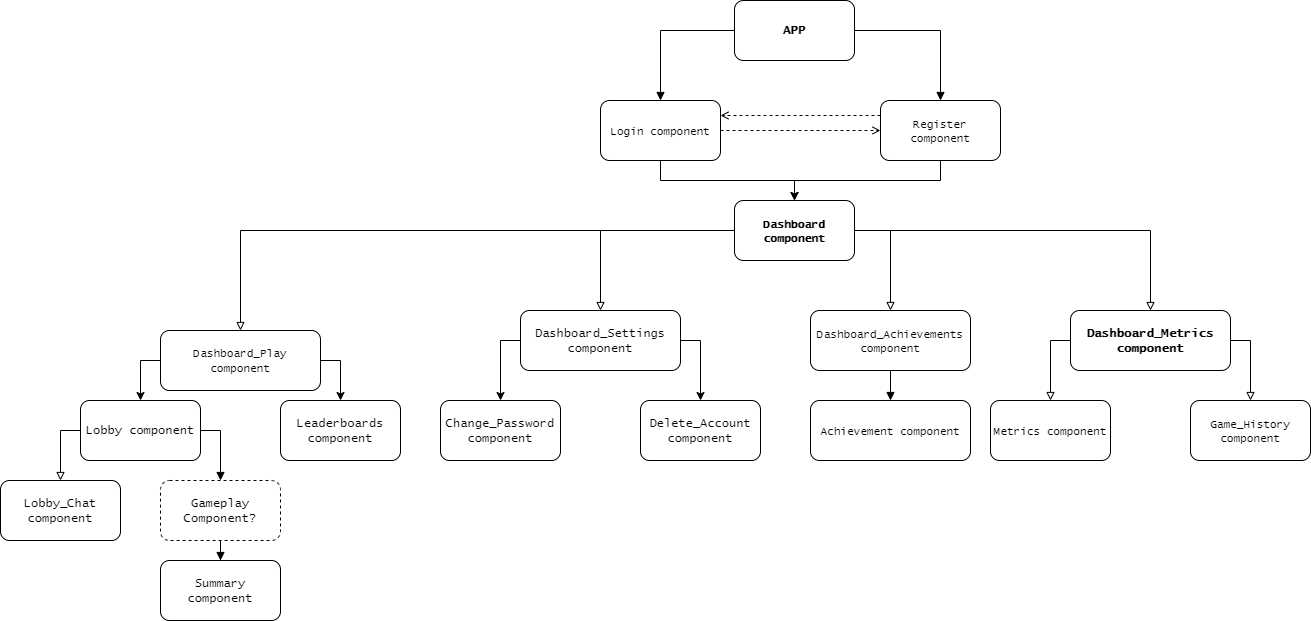
\includegraphics[width=1\linewidth]{images/react_comp_diagram.png}    

    \caption{React Component Diagram showing the hierarchy of the components in the web app, as well as the interactions between them. Arrows with a full black head means that the parent component navigates to the child component. Arrows with an open head means that the parent component is made up of the child components.}

    % use the notation fig:name to cross reference a figure
    \label{fig:react} 
\end{figure}

\section{The Chrome Extension}
Talk about the implementation of the extension


%==================================================================================================================================
\chapter{Evaluation} 
briefly mention participants, and the limitations that we had when trying to evaluate the project

\section{User Knowledge Of Targeted Advertising System}
Explain how we evaluate this, include statistical analysis with corresponding graphs.

\section{Gameplay Analysis}
Here is the analysis of the gameplay. For each game, for each player, look at their gameplay and try to get some meaning out of it.
Questions include:
 - What did users first try? Did they quickly realise better strategies?
 - What is the most common pattern seen amongst users (if any?)
 - Length of games for players that played more than one game
 - 

\section{System Usability}
After playing the game, participants were asked to answer 10 questions taken from the SUS questionnaire (CITE) to evaluate the usability of the system. To analyze the responses we ... *explain method*. Explain and 
interpret results. 

%==================================================================================================================================
\chapter{Conclusion}    

\section{Summary}
Summarise the whole project for a lazy reader who didn't read the rest (e.g. a prize-awarding committee).

\section{Limitations}
Explain what were the limitations in this project, what could be done differently? 
Limitations:
 - tracker list not exhaustive
 - Identifying and categorising ads is difficult, limited to Google's doubleclick ads

\section{Future Work}
For someone taking this project forward:
 - Explore more patterns for identifying adverts
 - Add more game modes and achievements
 - Maybe implement a new feature (look at Tally saves the internet)

\section{Final Reflections?}
Not sure if this paragraph will be included in the end, but here reflect on the project, did you learn anything new? Was it challenging? Refer from the notebook.

%==================================================================================================================================
%
% 
%==================================================================================================================================
%  APPENDICES  

\begin{appendices}

\chapter{Appendices}

\section{Ethics Checklist}
\begin{figure}
    \centering
    
\includegraphics{images/Ethics_Checklist.pdf}    

    \caption{Signed ethics checklist for the project.}

    % use the notation fig:name to cross reference a figure
    \label{fig:ethics} 
\end{figure}


\end{appendices}

%==================================================================================================================================
%   BIBLIOGRAPHY   

% The bibliography style is abbrvnat
% The bibliography always appears last, after the appendices.

\bibliographystyle{abbrvnat}

\bibliography{l4proj}

\end{document}
